\documentclass[a4paper,11pt]{article}
\usepackage[utf8]{inputenc}
\usepackage{graphicx}
\usepackage{textcomp}
\usepackage{gensymb}
\usepackage{cancel}
\usepackage{fancyhdr}
\usepackage{siunitx}
\usepackage{float}
\usepackage[labelfont=bf]{caption}
\usepackage[colorlinks=true,linkcolor=blue,urlcolor=blue,bookmarksopen=true]{hyperref}
\usepackage{subcaption}
\usepackage{amsmath}
\usepackage{amssymb}
\usepackage{booktabs}
\usepackage{bm}
\usepackage[margin=1in]{geometry}
\usepackage{setspace}

\usepackage[english]{babel}
\usepackage{amsthm}
\usepackage[noabbrev,capitalize,nameinlink]{cleveref}

\usepackage{enumitem}

\theoremstyle{plain}
\newtheorem*{thm}{Theorem}
\newtheorem*{cor}{Corollary}
\newtheorem{lem}{Lemma}
\newtheorem*{ax}{Axiom}

\theoremstyle{definition}
\newtheorem{definition}{Definition}
\newtheorem*{ex}{Example}
\newtheorem*{soln}{Solution}

\theoremstyle{remark}
\newtheorem*{rmk}{Remark}

\setlength{\parindent}{5ex}
\setlength{\headheight}{22pt}

\pagestyle{fancy}
\fancyhf{}
\rhead{CTA200} % Course Code
\lhead{Ian Niebres} % Name
\chead{\Large{\textbf{Assignment 3}}} % Title (Problem Set #)

\title{CTA200 2022 Assignment 3} % Title again
\author{Ian Niebres\\Tuesday, May 10 2022} % due date
\date{} 
\onehalfspacing
\begin{document}
\maketitle
\section*{Question 1}
%------------------------------------------------------------------%
%                           Question 1                             %
%------------------------------------------------------------------%
\quad\quad In this question, we iterated the equation $z_{n+1} = z_n^{\; 2} + c$ for
each point $c = x+iy$ in the complex plane for $-2 < x < 2$ and 
$-2 < y < 2$. A function called \texttt{iterate} was written
in the file \texttt{iteration.py} which performs this iteration
\texttt{N} times given an initial $z_0 = 0$ and $c = x+iy$.
This function returns the values of $z$, its modulus,
and the iteration number (at which it diverges, if it diverges).

Two
arrays were made, called \texttt{x\_vals} and \texttt{y\_vals},
using \texttt{numpy.arange} that contain 400 values from -2 to 2
equally spaced apart. The function \texttt{numpy.meshgrid}
was used with these arrays to create a
mesh grid of \texttt{x} and \texttt{y} values to be used
for plotting. A third array (called \texttt{zz}), for the third axis, was created
with all elements 0
with the same shape as the \texttt{x} and \texttt{y} arrays.
Using a double \texttt{for} loop, the elements of this third
array was filled with the last element returned by the
iteration value for each \texttt{x} and \texttt{y}.

The function \texttt{numpy.nan\_to\_num} was used to change
all \texttt{NaN}s in the array to a value over a threshold number.
All values equal or below this threshold
number were considered stable, and given the element corresponding
to the value's index was changed to 1. 
All values over this threshold number were considered to be
divergent, and given a value of 0.
At this point, we have enough to plot using \texttt{pyplot.imshow}
from \texttt{matplotlib}. A greyscale colourmap was used since
the data is binary. \cref{q1:1} was created where black shows
stability of the iteration with $c = x+iy$. White shows divergence.

The \texttt{iterate} function was changed, so that it now tracks
the iteration number at which it diverges. This was done by
using \texttt{numpy.where}, and searching for values at which the
modulus was
above the threshold. Since the function returns
the index, it was trivial to obtain the iteration number
at which it diverged. A copy of
the \texttt{zz} array of 0s was made, and updated with
this iteration number at divergence. A new plot, \cref*{q1:2}, was made
which shows the number of iterations it took for $z$ to diverge.
Note, 0 means the function does not diverge.

\begin{figure}[H]
    \centering
    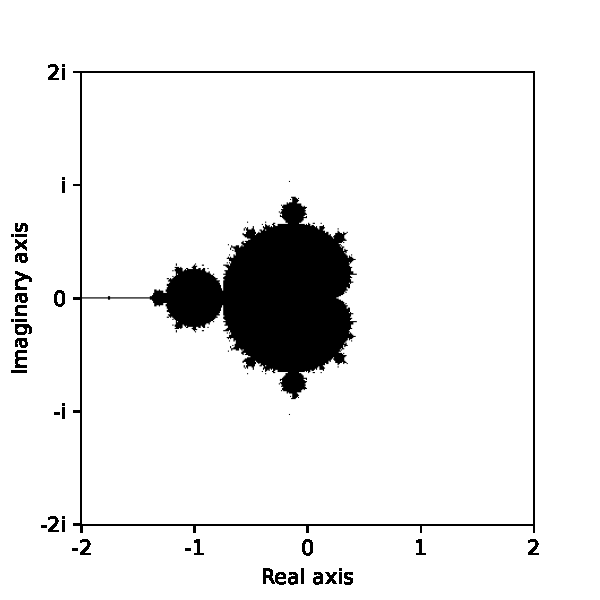
\includegraphics[width=0.65\linewidth]{../plots/a3q1_1.pdf}
    \caption{$x, y$ values used in the iteration of $z_{n+1}
    = z_n^{\; 2} + c$ where $c = x+iy$. Black points
    are bounded, white points diverge.}
    \label{q1:1}
\end{figure}
\begin{figure}[H]
    \centering
    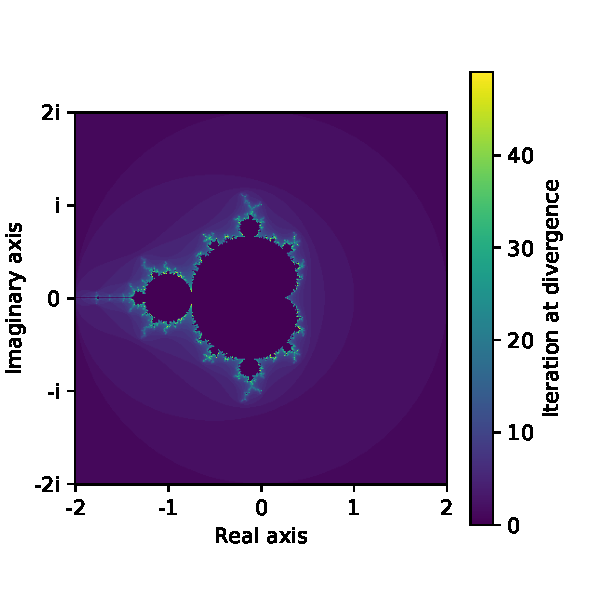
\includegraphics[width=0.65\linewidth]{../plots/a3q1_2.pdf}
    \caption{Same as \cref{q1:1}, but plot now shows the number of
    iterations before divergence.}
    \label{q1:2}
\end{figure}

\section*{Question 2}
%------------------------------------------------------------------%
%                           Question 2                             %
%------------------------------------------------------------------%
In this question, we wish to solve Lorenz' equations,
\begin{align}
    \dot{X} &= -\sigma(X+Y) \label{q2:eq1}\\
    \dot{Y} &= rX - Y - XZ\\
    \dot{Z} &= -bZ + XY \label{q2:eq3}
\end{align}
where $\sigma, r, b$ are the Prandtl number, the Rayleigh number, and
a length scale. Note that these are all dimensionless parameters. 
We will be using \texttt{solve\_ivp} from the package 
\texttt{scipy.integrate}.

\subsection*{Task 1}
Firstly, the constants (parameters) were assigned values
\texttt{[sigma, r, b]} = \texttt{[10., 28., 8./3.]}. 
As well, tolerances to be used for the \texttt{solve\_ivp}
function were defined. Lastly, the initial conditions
\texttt{W0 = [0., 1., 0.]} were defined. A function, \texttt{lorenz},
was written to be used
in \texttt{solve\_ivp}. This function is of
the right hand side of the ODEs in \cref{q2:eq1} to \cref{q2:eq3}.

\subsection*{Task 2}
Another function, called \texttt{solve\_lorenz}, was made,
which takes in a list of the initial conditions, and returns
the solved ODEs using \texttt{solve\_ivp}, in conjunction with
the previously assigned variables and tolerances in Task 1.

\subsection*{Task 3}
We were tasked to recreate Figure 1 from
\href{https://journals.ametsoc.org/view/journals/atsc/20/2/1520-0469_1963_020_0130_dnf_2_0_co_2.xml?tab_body=pdf}
{Lorenz' original paper}. The recreated figure is \cref{q2:1}. This
plot was made using \texttt{pyplot} from
\texttt{matplotlib}. This figure is a plot of Y values of the
numerical solution to the ODEs in \cref{q2:eq1} to \cref{q2:eq3}.



\subsection*{Task 4}
We were then tasked to recreate Figure 2, which are phase space
plots in the Y-X and Y-Z plane. Similar to what we did in Task 1,
but instead we are looking through iterations
1400 to 1900. See \cref{q2:2} and plotting different
values on the axes.

\subsection*{Task 5}
Now we wish to perturb the initial conditions
a small amount, and look at how the solution changes
over time. This was done by perturbing \texttt{W0 $\to$ W0'}
where \texttt{W0}' \texttt{= W0 + [0., 1.e-8, 0.]}. New solutions
were obtained using \texttt{W0}' as initial conditions
in the \texttt{solve\_lorenz} function. 
The distance between the two solutions \texttt{W} and \texttt{W'}
were calculated using the equation,
$\Delta x = \sqrt{(X-X')^2 + (Y-Y')^2 + (Z-Z')}$, where
$(X,Y,Z)$ and $(X', Y', Z')$ are the solutions to the Lorenz
equations with \texttt{W0} and \texttt{W0'} initial conditions,
respectively. The distance was then plotted
on a semilog plot using \texttt{pyplot.semilogy}, where
the time on the $x$-axis is linear, and the distance
on the $y$-axis is logarithmic. See \cref{q2:3}.

\begin{figure}[H]
    \centering
    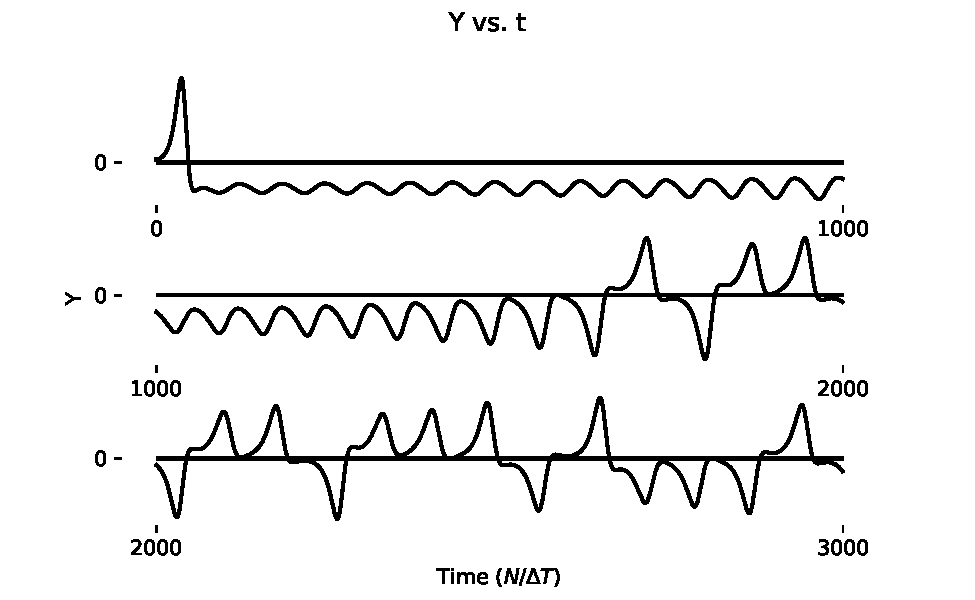
\includegraphics[width=\linewidth]{../plots/a3q2_y_vs_t.pdf}
    \caption{Plots of Y values of the
    numerical solution to the ODEs in \cref{q2:eq1} to \cref{q2:eq3}.
    Top: first 1000 iterations. Middle: iteration 1000 to
    2000. Bottom: iteration 2000 to 3000.}
    \label{q2:1}
\end{figure}

\begin{figure}[H]
    \centering
    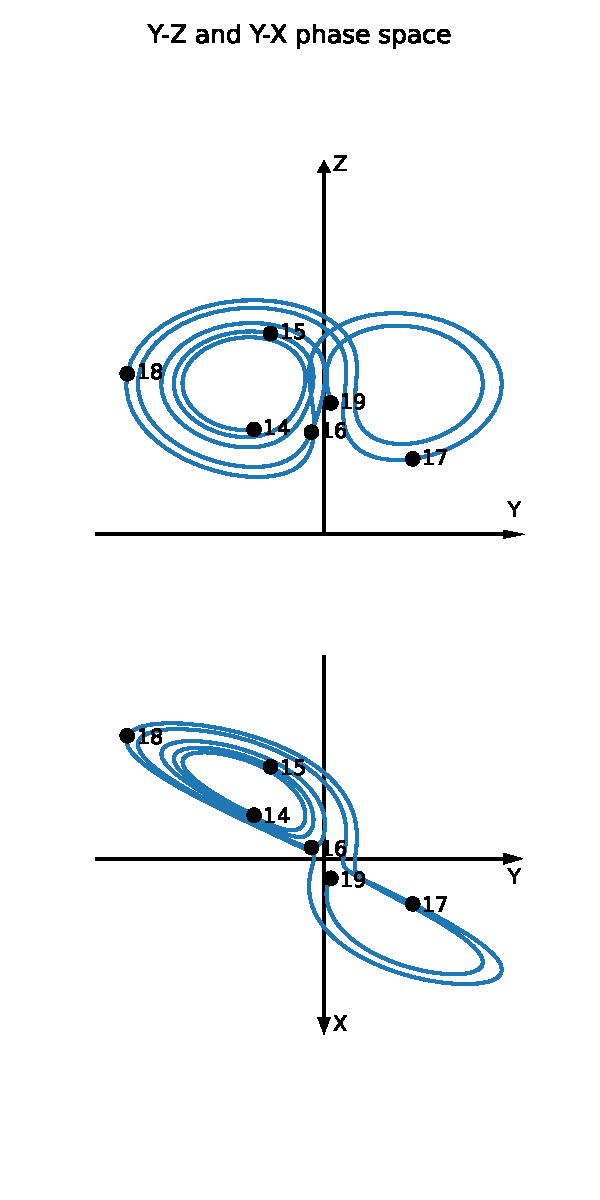
\includegraphics[width=0.6\linewidth]{../plots/a3q2_phase.pdf}
    \caption{Phase space plots of the
    numerical solution to the ODEs in \cref{q2:eq1} to \cref{q2:eq3}.
    Note, markers labeled
    14 to 19 indicate the solution at
    iterations 1400 to 1900, respectively. Top: Y-Z.
    2000. Bottom: Y-X phase space.}
    \label{q2:2}
\end{figure}

\begin{figure}[H]
    \centering
    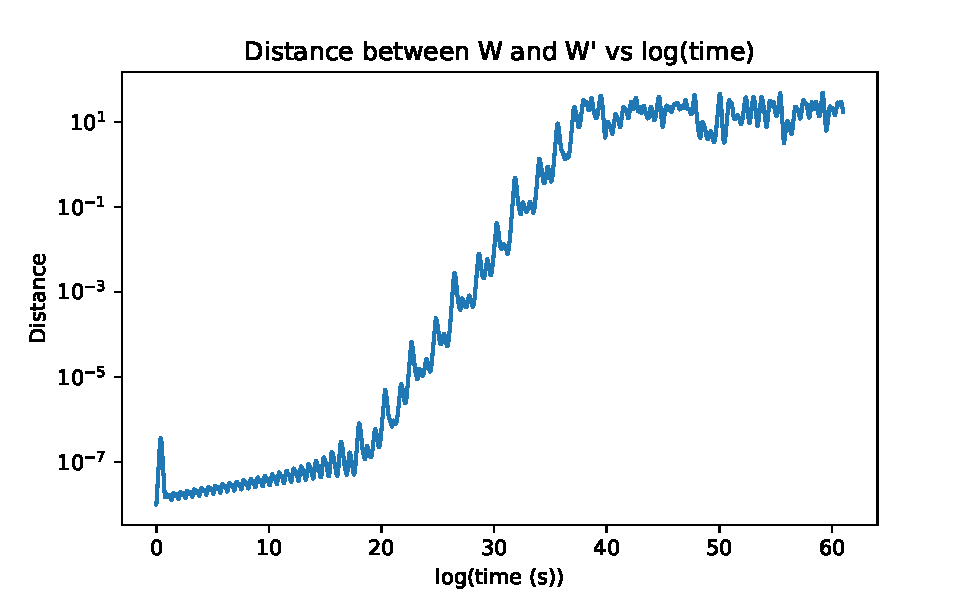
\includegraphics[width=\linewidth]{../plots/a3q2_dist_vs_t.pdf}
    \caption{Distance between solutions \texttt{W} and \texttt{W'}
    with respective initial conditions \texttt{W0} and \texttt{W0'}
    as a function of time.}
    \label{q2:3}
\end{figure}

\end{document}